\clearpage{}

\chapter{Queue evaluation Results}
\section{\label{sec:appendix-llic-performance}Results of Inner Experiments (\LL/\IC Evaluation)}

This appendix shows the results obtained by executing the Inner Experiments for the evaluation of the \LL/\IC objects, following the methodology suggested by Georges, Buytaert, and Eeckout~\cite{DBLP_conf_oopsla_GeorgesBE07}.

\begin{figure}[ht]
  \centering
  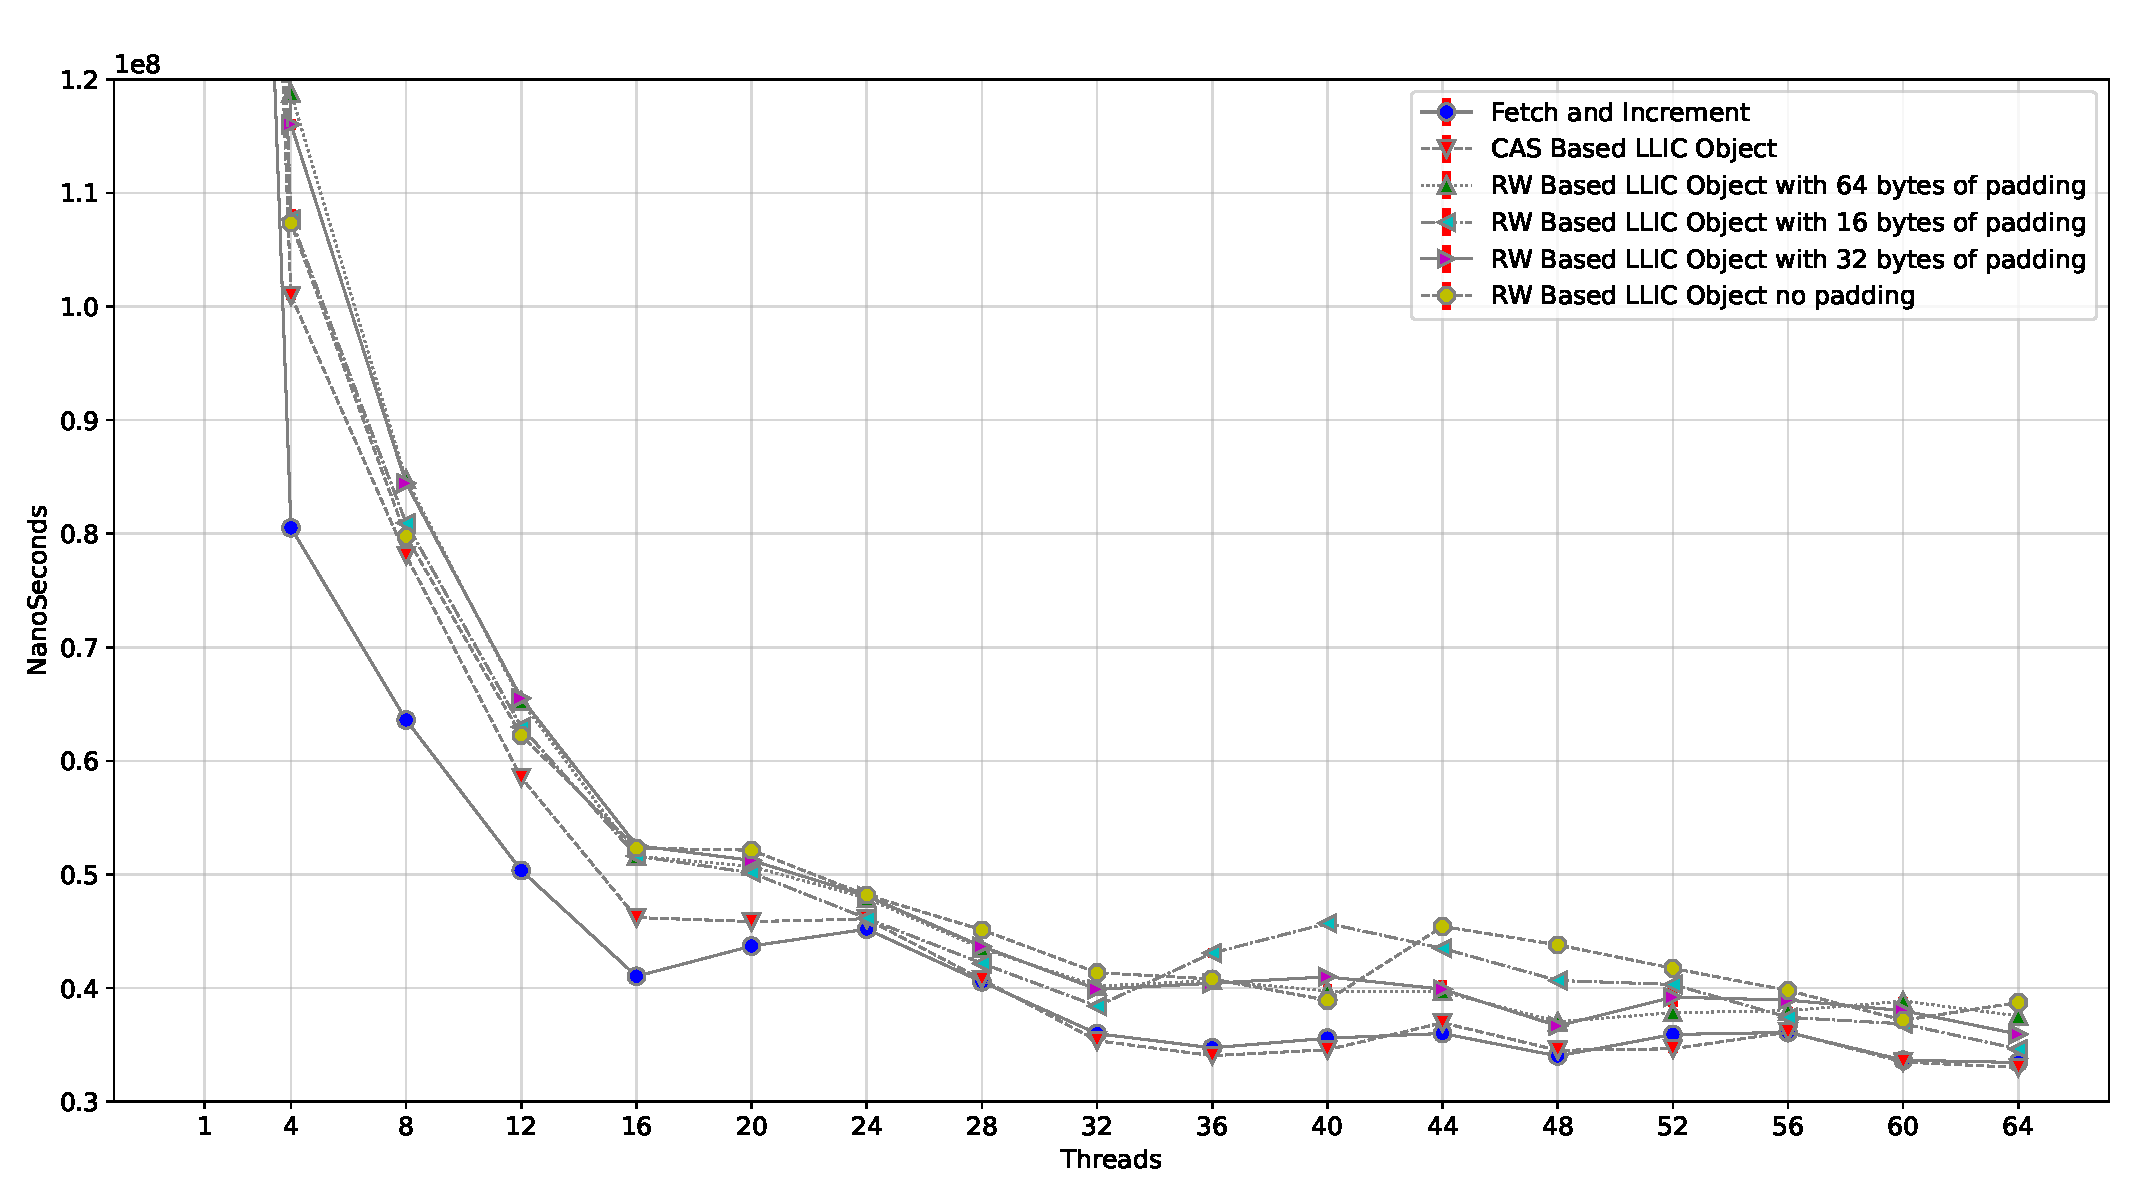
\includegraphics[scale=0.4]{contents/backmatter/evaluation/llic_64_insert_extract.pdf}
  \caption{\label{fig:appx-llic-64-insert-extract} 1,000,000 Interspersed Takes and Puts (CAS vs FAI) for 64 threads.}
\end{figure}


\begin{table}[!ht]
\centering\resizebox{\textwidth}{!}{\begin{tabular}{lrrrrrr}
\toprule
 & Fetch and Increment & CAS LL/IC & RW LL/IC 64 padding & RW LL/IC 16 padding & RW LL/IC 32 padding & RW LL/IC no padding \\
\midrule
\textbf{1} & 288860972.63 & 305638864.47 & 317065162.60 & 319755230.40 & 324187867.90 & 320378736.50 \\
\textbf{4} & 80506440.00 & 100958610.23 & 118799737.40 & 107684065.93 & 116027730.73 & 107367825.10 \\
\textbf{8} & 63599707.47 & 78075928.57 & 84805029.10 & 80927260.60 & 84444217.30 & 79758733.07 \\
\textbf{12} & 50347568.87 & 58526625.20 & 65273976.33 & 62985744.70 & 65516543.10 & 62251471.77 \\
\textbf{16} & 41037828.93 & 46203364.33 & 51603157.93 & 51627402.33 & 52549893.80 & 52305099.07 \\
\textbf{20} & 43698354.07 & 45852623.00 & 50705047.53 & 50136623.90 & 51232438.97 & 52131764.40 \\
\textbf{24} & 45187224.67 & 46074348.43 & 47896947.17 & 46134113.00 & 48109941.77 & 48176109.00 \\
\textbf{28} & 40547444.73 & 40755668.37 & 43482972.33 & 42171177.13 & 43660332.43 & 45119529.33 \\
\textbf{32} & 35988846.27 & 35367188.00 & 40166244.37 & 38405117.57 & 39891455.73 & 41353746.77 \\
\textbf{36} & 34734531.67 & 34048104.30 & 40661526.40 & 43080326.90 & 40424838.03 & 40796560.43 \\
\textbf{40} & 35586323.23 & 34568989.23 & 39735940.17 & 45696269.77 & 40990485.80 & 38923483.30 \\
\textbf{44} & 36000699.17 & 36938976.17 & 39689813.13 & 43486986.73 & 39893678.63 & 45420477.57 \\
\textbf{48} & 34018945.07 & 34521533.77 & 37031091.27 & 40663404.70 & 36665244.53 & 43799081.63 \\
\textbf{52} & 35914989.23 & 34660215.90 & 37839803.70 & 40314233.27 & 39197357.90 & 41730669.73 \\
\textbf{56} & 36094405.17 & 36113970.37 & 38005800.77 & 37420952.30 & 38938837.97 & 39787863.63 \\
\textbf{60} & 33648086.47 & 33491633.80 & 38858203.27 & 36847570.77 & 38009665.63 & 37164143.80 \\
\textbf{64} & 33447182.50 & 33003608.20 & 37543791.23 & 34631263.33 & 35936880.00 & 38732530.37 \\
\bottomrule
\end{tabular}}
\caption{Mean times for LL/IC experiemnt}
\label{table:llic-times}
\end{table}

\begin{table}[!ht]
\centering\resizebox{\textwidth}{!}{\begin{tabular}{lrrrrrr}
\toprule
 & Fetch and Increment & CAS LL/IC & RW LL/IC 64 padding & RW LL/IC 16 padding & RW LL/IC 32 padding & RW LL/IC no padding \\
\midrule
\textbf{1} & 0.00 & -5.81 & -9.76 & -10.70 & -12.23 & -10.91 \\
\textbf{4} & 0.00 & -25.40 & -47.57 & -33.76 & -44.12 & -33.37 \\
\textbf{8} & 0.00 & -22.76 & -33.34 & -27.24 & -32.77 & -25.41 \\
\textbf{12} & 0.00 & -16.25 & -29.65 & -25.10 & -30.13 & -23.64 \\
\textbf{16} & 0.00 & -12.59 & -25.75 & -25.80 & -28.05 & -27.46 \\
\textbf{20} & 0.00 & -4.93 & -16.03 & -14.73 & -17.24 & -19.30 \\
\textbf{24} & 0.00 & -1.96 & -6.00 & -2.10 & -6.47 & -6.61 \\
\textbf{28} & 0.00 & -0.51 & -7.24 & -4.00 & -7.68 & -11.28 \\
\textbf{32} & 0.00 & 1.73 & -11.61 & -6.71 & -10.84 & -14.91 \\
\textbf{36} & 0.00 & 1.98 & -17.06 & -24.03 & -16.38 & -17.45 \\
\textbf{40} & 0.00 & 2.86 & -11.66 & -28.41 & -15.19 & -9.38 \\
\textbf{44} & 0.00 & -2.61 & -10.25 & -20.79 & -10.81 & -26.17 \\
\textbf{48} & 0.00 & -1.48 & -8.85 & -19.53 & -7.78 & -28.75 \\
\textbf{52} & 0.00 & 3.49 & -5.36 & -12.25 & -9.14 & -16.19 \\
\textbf{56} & 0.00 & -0.05 & -5.30 & -3.68 & -7.88 & -10.23 \\
\textbf{60} & 0.00 & 0.46 & -15.48 & -9.51 & -12.96 & -10.45 \\
\textbf{64} & 0.00 & 1.33 & -12.25 & -3.54 & -7.44 & -15.80 \\
\bottomrule
\end{tabular}}
\caption{Percentage improvement of LL/IC objects respect to \FAI from 1 to 64 threads of execution.}
\label{table:appx-llic-percentages}
\end{table}


\section{\label{sec:appendix-inner-queues}Results of Inner Experiments (Module Queue Variants)}

\begin{figure}[ht]
  \centering
  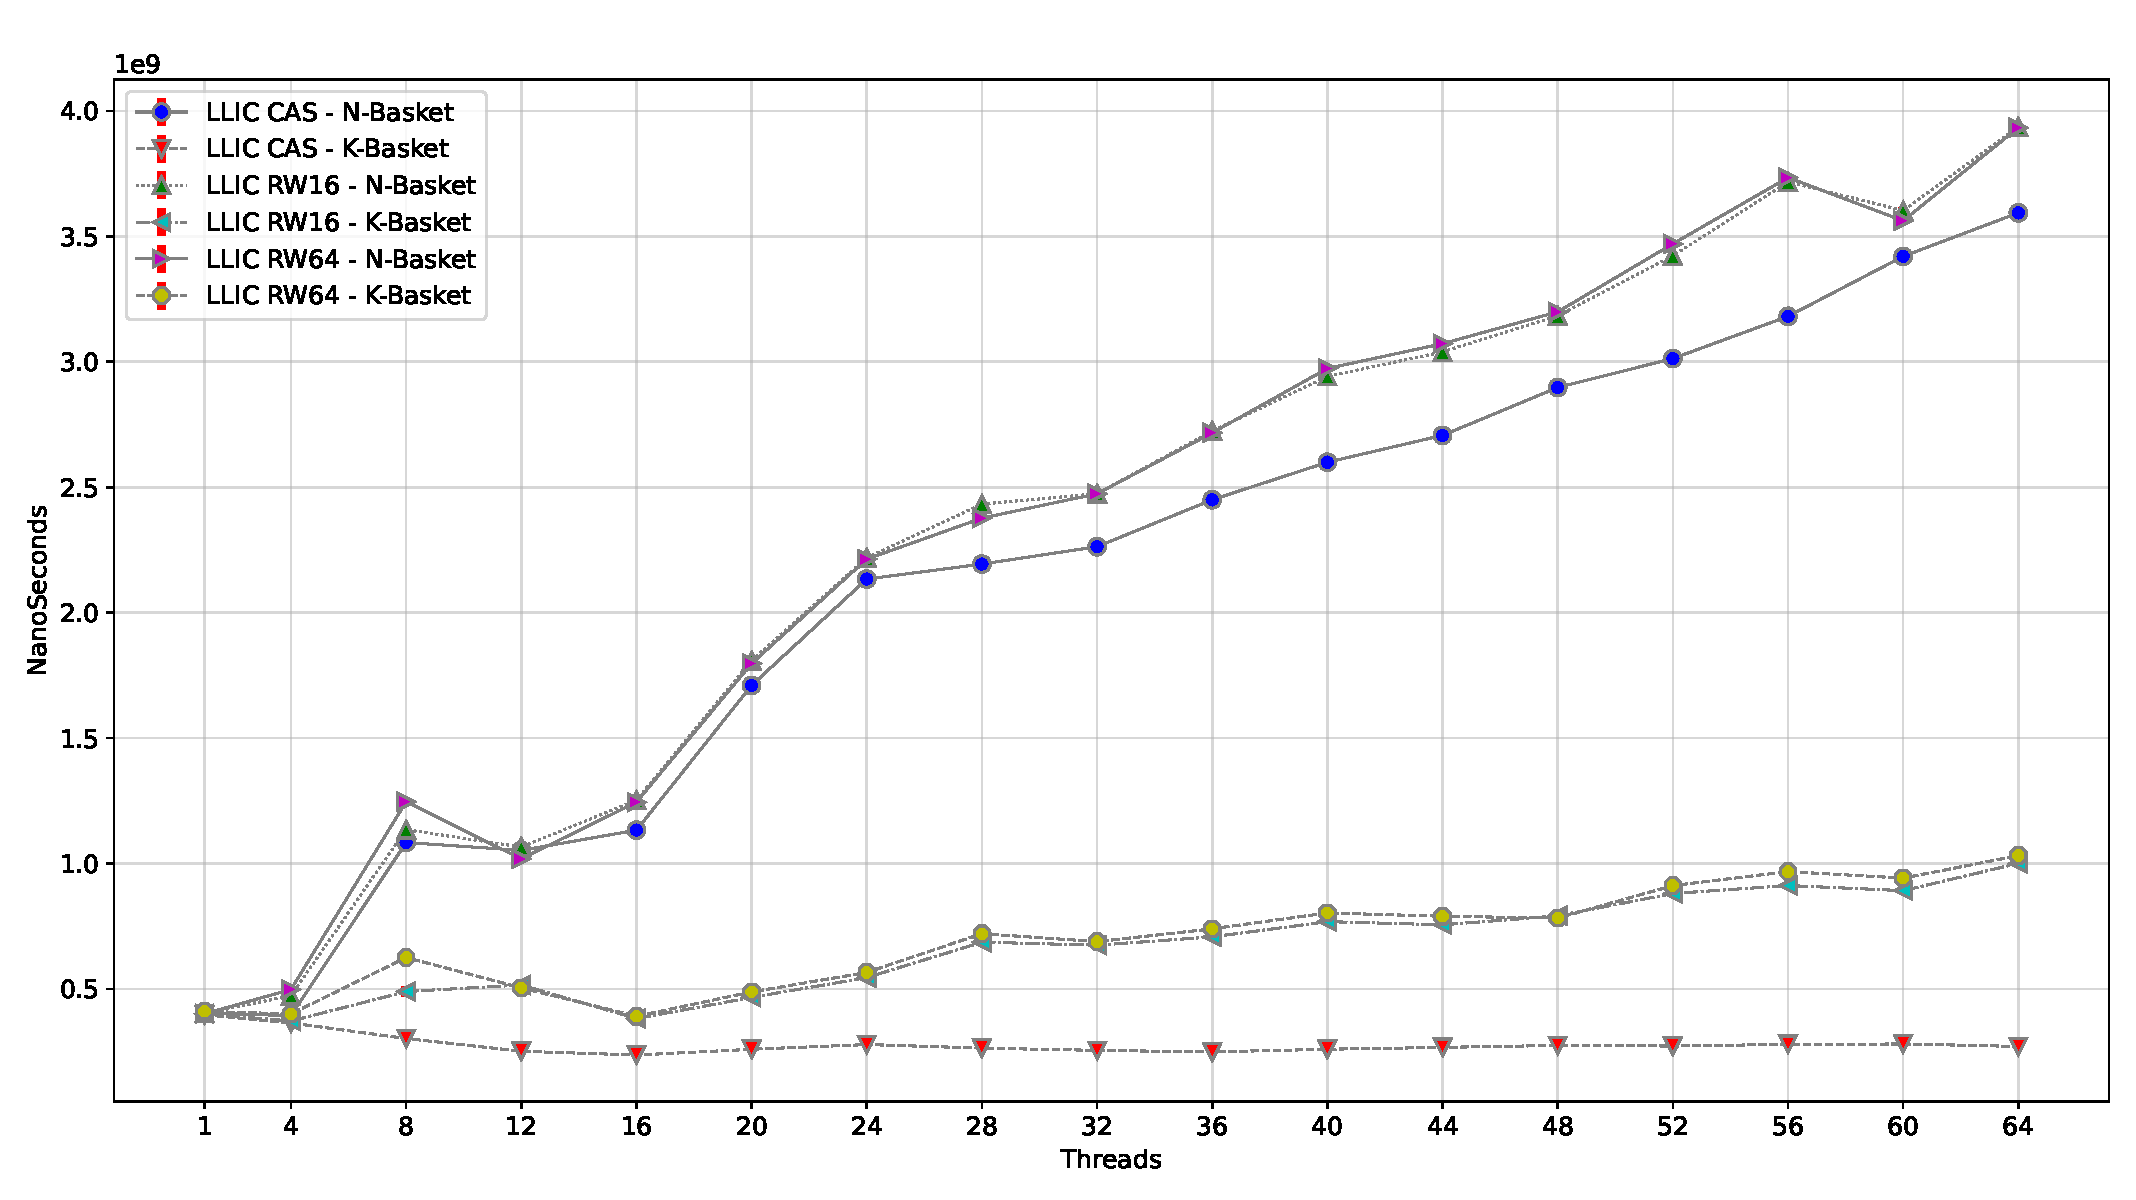
\includegraphics[scale=0.4]{contents/backmatter/evaluation/64_inner_enq_deq_all.pdf}
  \caption{\label{fig:appx-64_inner_enq_deq_all} 1,000,000 interspersed enqueue - dequeue calls for 64 threads.}
\end{figure}

\begin{table}[!ht]
\centering\resizebox{\textwidth}{!}{\begin{tabular}{lrrrrrr}
\toprule
 & LLIC CAS - N-Basket & LLIC CAS - K-Basket & LLIC RW16 - N-Basket & LLIC RW16 - K-Basket & LLIC RW64 - N-Basket & LLIC RW64 - K-Basket \\
\midrule
\textbf{1} & -1.74 & 0.00 & -1.62 & -0.79 & -0.89 & -3.39 \\
\textbf{4} & -8.04 & 0.00 & -29.92 & -2.17 & -36.75 & -9.86 \\
\textbf{8} & -258.89 & 0.00 & -275.82 & -62.07 & -312.78 & -106.99 \\
\textbf{12} & -319.04 & 0.00 & -324.39 & -105.25 & -305.49 & -100.73 \\
\textbf{16} & -379.75 & 0.00 & -430.37 & -61.63 & -427.12 & -65.46 \\
\textbf{20} & -559.67 & 0.00 & -597.66 & -79.74 & -593.29 & -88.13 \\
\textbf{24} & -667.53 & 0.00 & -697.90 & -96.02 & -696.10 & -103.47 \\
\textbf{28} & -732.44 & 0.00 & -823.17 & -160.38 & -801.91 & -173.19 \\
\textbf{32} & -789.13 & 0.00 & -872.14 & -164.84 & -872.05 & -170.39 \\
\textbf{36} & -885.69 & 0.00 & -995.94 & -184.55 & -993.03 & -197.53 \\
\textbf{40} & -902.46 & 0.00 & -1034.40 & -196.16 & -1046.65 & -209.51 \\
\textbf{44} & -914.62 & 0.00 & -1039.46 & -183.09 & -1051.62 & -195.87 \\
\textbf{48} & -956.29 & 0.00 & -1060.54 & -188.44 & -1066.28 & -185.11 \\
\textbf{52} & -1007.88 & 0.00 & -1158.48 & -223.66 & -1176.07 & -235.25 \\
\textbf{56} & -1040.85 & 0.00 & -1233.05 & -227.03 & -1239.22 & -246.94 \\
\textbf{60} & -1120.14 & 0.00 & -1185.35 & -218.00 & -1170.88 & -235.85 \\
\textbf{64} & -1229.50 & 0.00 & -1356.19 & -270.04 & -1355.10 & -281.49 \\
\bottomrule
\end{tabular}}
\caption{Percentage improvement of Enqueue - Dequeue respect to LL/IC \CAS \& K-Basket from 1 to 64 threads of execution.}
\label{table:appx-64-inner-enq-deq-percentages}
\end{table}

\begin{table}[!ht]
\centering\resizebox{\textwidth}{!}{\begin{tabular}{lrrrrrr}
\toprule
 & LLIC CAS - N-Basket & LLIC CAS - K-Basket & LLIC RW16 - N-Basket & LLIC RW16 - K-Basket & LLIC RW64 - N-Basket & LLIC RW64 - K-Basket \\
\midrule
\textbf{1} & 403837572.97 & 396923559.23 & 403364522.07 & 400055812.90 & 400458163.90 & 410361616.03 \\
\textbf{4} & 393072415.97 & 363825211.27 & 472695382.10 & 371714856.90 & 497516571.87 & 399706830.60 \\
\textbf{8} & 1083497864.53 & 301903826.67 & 1134626840.47 & 489293420.43 & 1246191018.60 & 624905787.60 \\
\textbf{12} & 1052047521.10 & 251061393.53 & 1065479541.67 & 515315431.30 & 1018033354.13 & 503958613.03 \\
\textbf{16} & 1132563585.47 & 236075970.90 & 1252081224.87 & 381578408.67 & 1244407677.97 & 390607216.17 \\
\textbf{20} & 1709842518.17 & 259198051.17 & 1808325283.23 & 465887426.90 & 1796996372.03 & 487635858.33 \\
\textbf{24} & 2133731012.70 & 278000991.57 & 2218159617.33 & 544932910.07 & 2213154726.97 & 565660003.90 \\
\textbf{28} & 2193455107.57 & 263495757.53 & 2432517335.17 & 686078560.50 & 2376492044.60 & 719843684.83 \\
\textbf{32} & 2262827345.93 & 254498662.33 & 2474083071.13 & 674008201.03 & 2473843065.13 & 688144066.47 \\
\textbf{36} & 2449877745.93 & 248545543.60 & 2723899346.60 & 707239057.03 & 2716683811.97 & 739506175.80 \\
\textbf{40} & 2599424591.43 & 259304569.17 & 2941545544.63 & 767947461.03 & 2973306680.03 & 802582429.10 \\
\textbf{44} & 2706567513.60 & 266755495.50 & 3039584219.03 & 755145375.97 & 3072020329.00 & 789260312.00 \\
\textbf{48} & 2897334261.40 & 274293059.03 & 3183274684.97 & 791166367.20 & 3199031929.60 & 782029672.97 \\
\textbf{52} & 3012856935.07 & 271947171.90 & 3422409173.57 & 880173001.43 & 3470237815.97 & 911715385.53 \\
\textbf{56} & 3181102862.03 & 278835375.93 & 3717005695.57 & 911886436.97 & 3734223566.20 & 967380566.13 \\
\textbf{60} & 3420201175.47 & 280311296.37 & 3602981476.13 & 891396736.43 & 3562427501.20 & 941420017.77 \\
\textbf{64} & 3593712103.47 & 270304602.33 & 3936145887.47 & 1000239685.37 & 3933207413.67 & 1031183359.33 \\
\bottomrule
\end{tabular}}
\caption{Mean times for Enqueue - Dequeue inner experiment for 64 threads.}
\label{table:appx-64-inner-enq-deq-times}
\end{table}


\section{\label{sec:appendix-outer-queue}Results of Outer Experiments}

\begin{figure}[ht]
  \centering
  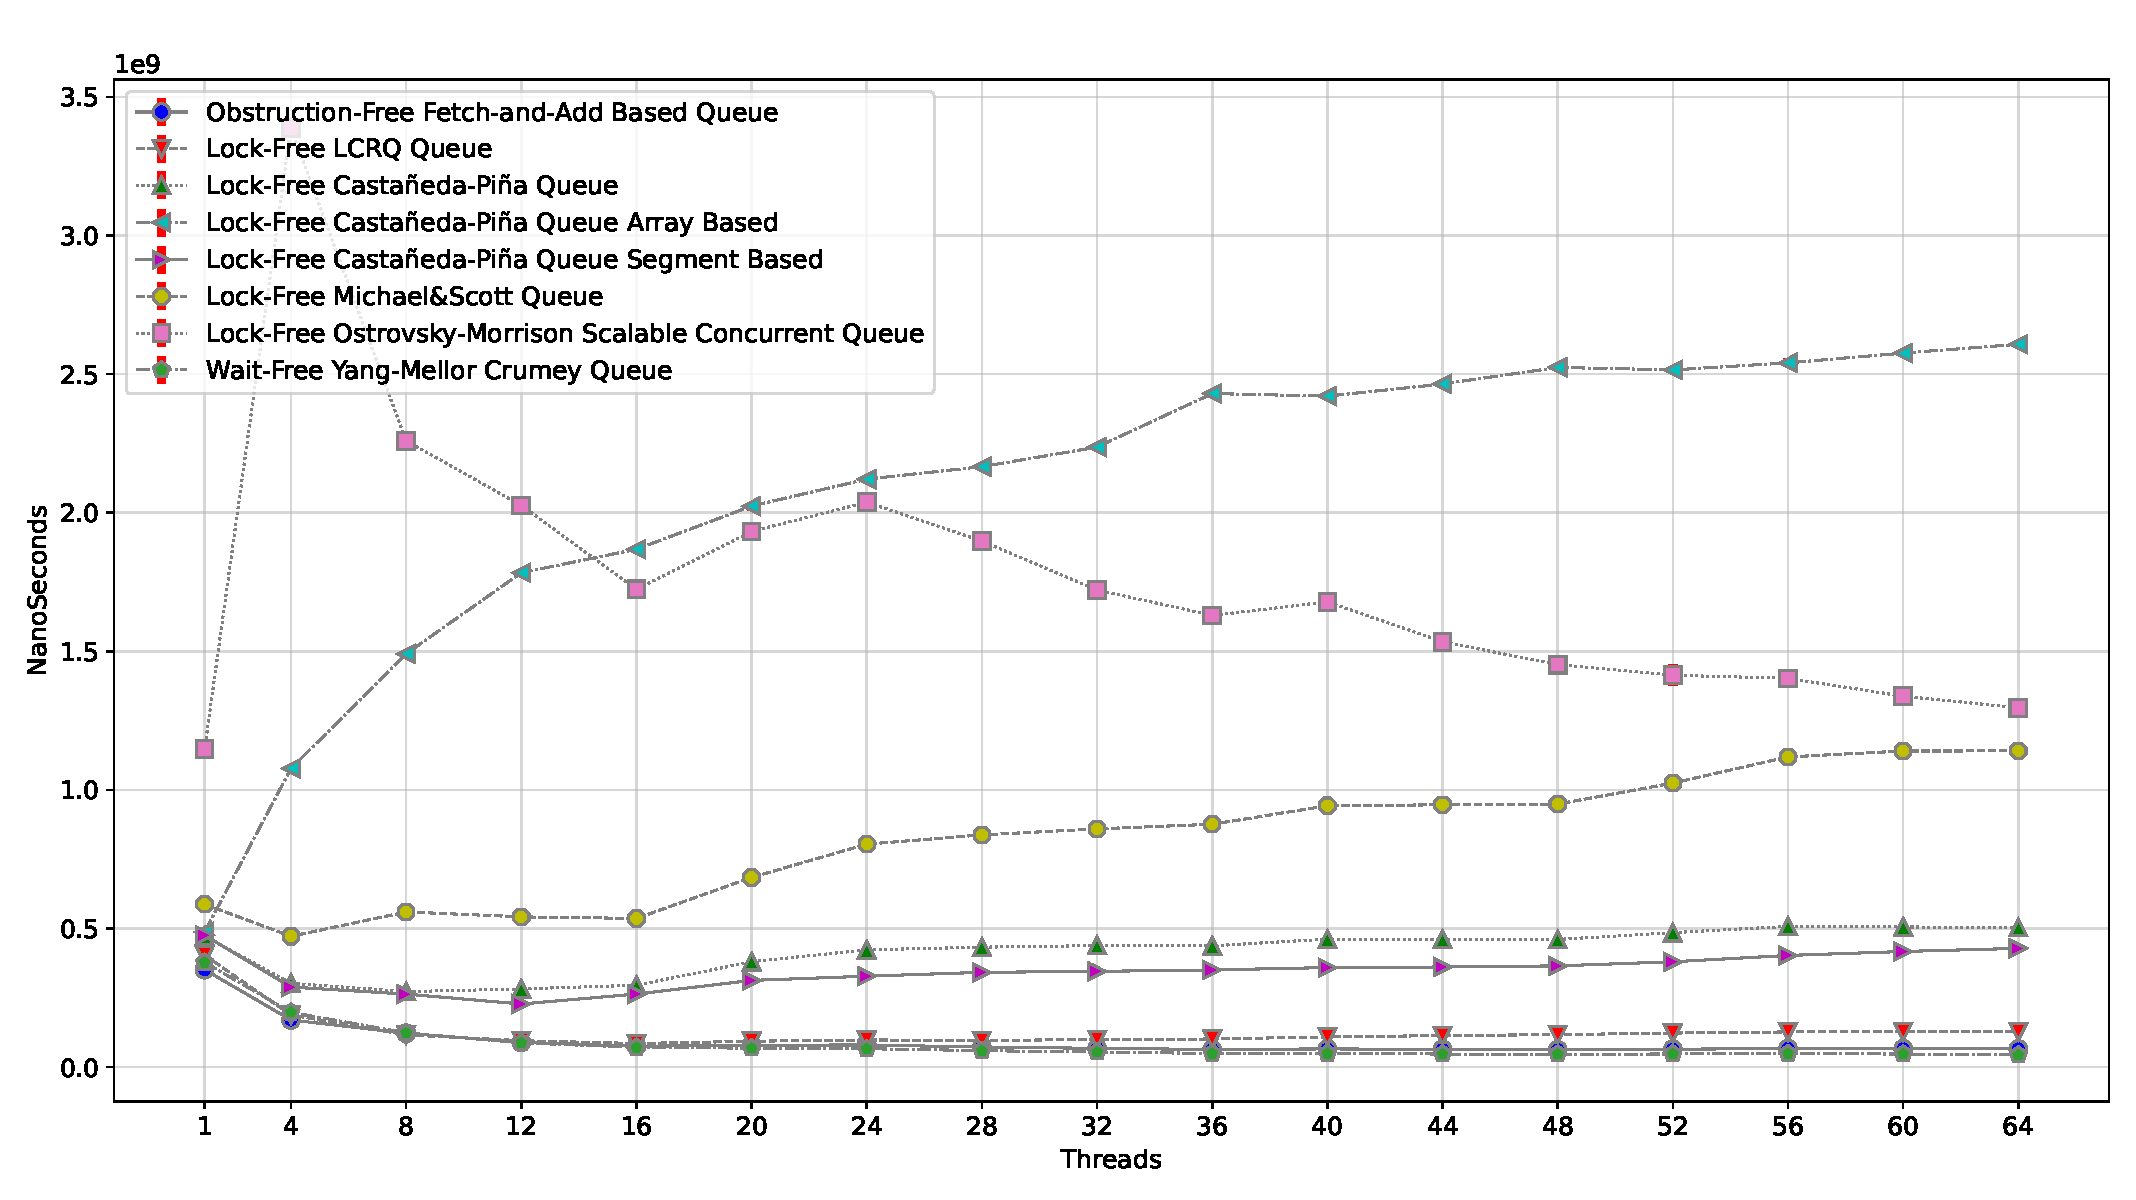
\includegraphics[scale=0.4]{contents/backmatter/evaluation/64_outer_enq_deq_all.pdf}
  \caption{\label{fig:appx-64-outer-enq-deq}1,000,000 of interspersed Enqueue - Dequeue calls for 64 threads.}
\end{figure}

\begin{table}[!ht]
\centering\resizebox{\textwidth}{!}{\begin{tabular}{lrrrrrrrr}
\toprule
 & Fetch-and-Add & LCRQ & Castañeda-Piña & Castañeda-Piña Array & Castañeda-Piña Segments & Michael and Scott & Ostrovsky-Morrison & YMC \\
\midrule
\textbf{1} & 351200027.63 & 403572408.43 & 472555550.90 & 487165396.30 & 475511479.40 & 587248865.70 & 1146251708.13 & 377297171.80 \\
\textbf{4} & 169692112.77 & 187820883.50 & 301829643.73 & 1077150109.93 & 288435581.67 & 471544279.67 & 3387292159.17 & 197394522.23 \\
\textbf{8} & 121854879.07 & 116026264.60 & 272038021.70 & 1490503277.57 & 263046870.43 & 559538345.73 & 2259382162.50 & 122918448.70 \\
\textbf{12} & 88994036.27 & 94770156.63 & 281703838.03 & 1783321075.57 & 227342770.57 & 541606321.37 & 2026162066.43 & 87396589.83 \\
\textbf{16} & 74776242.40 & 84622830.50 & 294978630.73 & 1867961323.20 & 263256036.93 & 535908982.53 & 1723493401.93 & 70816962.53 \\
\textbf{20} & 78627962.80 & 93050854.37 & 379995043.80 & 2023925634.47 & 312408909.57 & 684008030.47 & 1932146663.93 & 67941366.37 \\
\textbf{24} & 79543299.43 & 97720927.97 & 422919854.07 & 2120916067.10 & 327654824.50 & 803985551.10 & 2037756243.03 & 66012273.80 \\
\textbf{28} & 71817559.87 & 95509834.43 & 432414808.13 & 2166062984.03 & 341570968.90 & 837462016.30 & 1897402494.37 & 59065987.40 \\
\textbf{32} & 67443713.50 & 99412632.57 & 438538137.47 & 2236554396.10 & 345087614.40 & 859154816.23 & 1720945612.37 & 53669770.97 \\
\textbf{36} & 63240889.47 & 101217631.23 & 437121875.30 & 2429715567.90 & 350204025.40 & 875829430.07 & 1629208308.67 & 48970421.20 \\
\textbf{40} & 65311551.40 & 108716588.03 & 461605337.17 & 2420424604.93 & 358781500.57 & 942633485.97 & 1678287663.47 & 48899447.00 \\
\textbf{44} & 63473601.93 & 113385554.47 & 460308301.33 & 2464267895.70 & 360854102.40 & 946151498.10 & 1534113476.07 & 46628124.97 \\
\textbf{48} & 62148500.10 & 116865624.87 & 460302515.57 & 2523987255.27 & 364872124.93 & 948736421.87 & 1451514990.13 & 46240439.33 \\
\textbf{52} & 64238033.60 & 122543525.30 & 484756656.03 & 2514987713.47 & 379651287.00 & 1024468571.63 & 1413332353.37 & 47095151.57 \\
\textbf{56} & 66547657.57 & 126754099.80 & 507507288.80 & 2540588509.17 & 402499664.00 & 1118652395.07 & 1402048064.73 & 47973167.30 \\
\textbf{60} & 65885871.70 & 127109938.03 & 505315540.43 & 2575744556.40 & 416756883.57 & 1140158428.23 & 1337866333.20 & 46690629.67 \\
\textbf{64} & 65178512.30 & 126730354.90 & 502870762.67 & 2607573629.43 & 428069875.03 & 1140572453.10 & 1295963945.30 & 43235588.63 \\
\bottomrule
\end{tabular}}
\caption{Mean times for Enqueue - Dequeue outer experiment for 64 threads.}
\label{table:appx64-outer-enq-deq-times}
\end{table}

\begin{table}[!ht]
\centering\resizebox{\textwidth}{!}{\begin{tabular}{lrrrrrrrr}
\toprule
 & Fetch-and-Add & LCRQ & Castañeda-Piña & Castañeda-Piña Array & Castañeda-Piña Segments & Michael and Scott & Ostrovsky-Morrison & YMC \\
\midrule
\textbf{1} & 6.92 & -6.96 & -25.25 & -29.12 & -26.03 & -55.65 & -203.81 & 0.00 \\
\textbf{4} & 14.03 & 4.85 & -52.91 & -445.68 & -46.12 & -138.88 & -1616.00 & 0.00 \\
\textbf{8} & 0.87 & 5.61 & -121.32 & -1112.60 & -114.00 & -355.21 & -1738.11 & 0.00 \\
\textbf{12} & -1.83 & -8.44 & -222.33 & -1940.49 & -160.13 & -519.71 & -2218.35 & 0.00 \\
\textbf{16} & -5.59 & -19.50 & -316.54 & -2537.73 & -271.74 & -656.75 & -2333.73 & 0.00 \\
\textbf{20} & -15.73 & -36.96 & -459.30 & -2878.93 & -359.82 & -906.76 & -2743.84 & 0.00 \\
\textbf{24} & -20.50 & -48.03 & -540.67 & -3112.91 & -396.35 & -1117.93 & -2986.94 & 0.00 \\
\textbf{28} & -21.59 & -61.70 & -632.09 & -3567.19 & -478.29 & -1317.84 & -3112.34 & 0.00 \\
\textbf{32} & -25.66 & -85.23 & -717.10 & -4067.25 & -542.98 & -1500.82 & -3106.55 & 0.00 \\
\textbf{36} & -29.14 & -106.69 & -792.62 & -4861.60 & -615.13 & -1688.49 & -3226.92 & 0.00 \\
\textbf{40} & -33.56 & -122.33 & -843.99 & -4849.80 & -633.71 & -1827.70 & -3332.12 & 0.00 \\
\textbf{44} & -36.13 & -143.17 & -887.19 & -5184.94 & -673.90 & -1929.14 & -3190.10 & 0.00 \\
\textbf{48} & -34.40 & -152.73 & -895.45 & -5358.40 & -689.08 & -1951.75 & -3039.06 & 0.00 \\
\textbf{52} & -36.40 & -160.20 & -929.31 & -5240.23 & -706.14 & -2075.32 & -2901.01 & 0.00 \\
\textbf{56} & -38.72 & -164.22 & -957.90 & -5195.85 & -739.01 & -2231.83 & -2822.57 & 0.00 \\
\textbf{60} & -41.11 & -172.24 & -982.26 & -5416.62 & -792.59 & -2341.94 & -2765.39 & 0.00 \\
\textbf{64} & -50.75 & -193.12 & -1063.09 & -5931.08 & -890.09 & -2538.04 & -2897.45 & 0.00 \\
\bottomrule
\end{tabular}}
\caption{Percentage improvement of Enqueue - Dequeue respect to Yang and Mellor-Crummey Queue from 1 to 64 threads of execution.}
\label{table:appx-64-outer-enq-deq-percentages}
\end{table}





%%% Local Variables:
%%% mode: LaTeX
%%% TeX-master: "../../main"
%%% End:
